\documentclass[tikz,border=3pt]{standalone}
\usetikzlibrary{shapes.geometric}
% \usetikzlibrary{arrows.meta}
\usetikzlibrary{decorations.text}
\definecolor{darkgreen}{RGB}{0,100,0}

\begin{document}
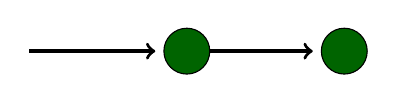
\begin{tikzpicture}[square/.style={regular polygon,regular polygon sides=4}]
    
    \node[circle, fill=darkgreen, draw=black, text width=0.3cm]  at (0, 0) (A) {};
    \node[circle, fill=darkgreen, draw=black, text width=0.3cm]  at (2, 0) (B) {};
    
    
    \draw (-2,0) edge[->, very thick] (-0.4,0) ;
    \draw (A) edge[->, very thick] (1.6,0) ;
    
\end{tikzpicture}
\end{document}
